\documentclass{article}
\usepackage[margin=1in]{geometry}
\usepackage{url}
\usepackage{forest}
\usepackage{tabu}
\usepackage{listings}
\usepackage{amsmath}
\usepackage{amsfonts}
\usepackage{float}
\usepackage{color}
\usepackage{multicol}
\usepackage{textcomp}
\usepackage[normalem]{ulem}
\usepackage[colorlinks = true,
            linkcolor = blue,
            urlcolor  = blue,
            citecolor = blue,
            anchorcolor = blue]{hyperref}
\usepackage{subfig}
\usepackage{mdframed}
\usepackage[font=small,labelfont=bf]{caption}

\title{Tools For Data Science: Optimizing Team USA's Gymnastics Roster for the Paris 2024 Olympics \\ \textbf{Executive Summary}}
\author{Rami Pellumbi\thanks{M.S., Statistics \& Data Science}}
\date{\today}

\begin{document}
\maketitle
\newpage
\paragraph{Introduction} This report outlines a sophisticated system designed to optimize Team USA's roster selection for the Paris 2024 Olympics in Men's and Women's Artistic Gymnastics. Utilizing a blend of statistical modeling and simulation techniques, the system provides a user interface that empowers users to have a data-driven approach to formulating competitive team compositions.

\paragraph{Methodology}
At the heart of the system are linear regression models for each gender-apparatus pair, predicting athletes' execution scores based on difficulty scores and athlete names. These models are grounded in rigorous data analysis, ensuring robust and relevant insights for team selection.

\paragraph{Data Integrity} A meticulous data exploration and cleansing process was undertaken to ensure the accuracy of the models. This included addressing inconsistencies and duplicate athlete names, resulting in a highly reliable dataset.

\paragraph{Model Performance} The linear regression models, chosen for their simplicity and interpretability, demonstrate satisfactory performance. This is evidenced by reasonable 
$R^2$ values across different apparatuses and genders, indicating a good fit with the data.

\paragraph{Application of the Model}
Monte Carlo simulations, based on the model's predictions, are used to forecast the outcomes of various Olympic events. 
These simulations offer a view of simulated medal counts for allocated teams. The 
client application is the real strength of the system, offering a user-friendly
interface for exploring the results of the simulations. Figures \ref{fig:sim_runner} and \ref{fig:sim_results} provide
examples of the application's output.

\paragraph{Analysis of Results}
The results from these simulations provide strategic insights into team composition, highlighting which athletes have the greatest potential impact on Team USA's success.

\paragraph{Implications and Recommendations}
The system offers a data-driven approach to team selection, allowing coaches and decision-makers to make informed choices. Beyond gymnastics, this methodology has potential applications in other sports and fields where team composition is crucial.


\begin{figure}[H]
    \centering
    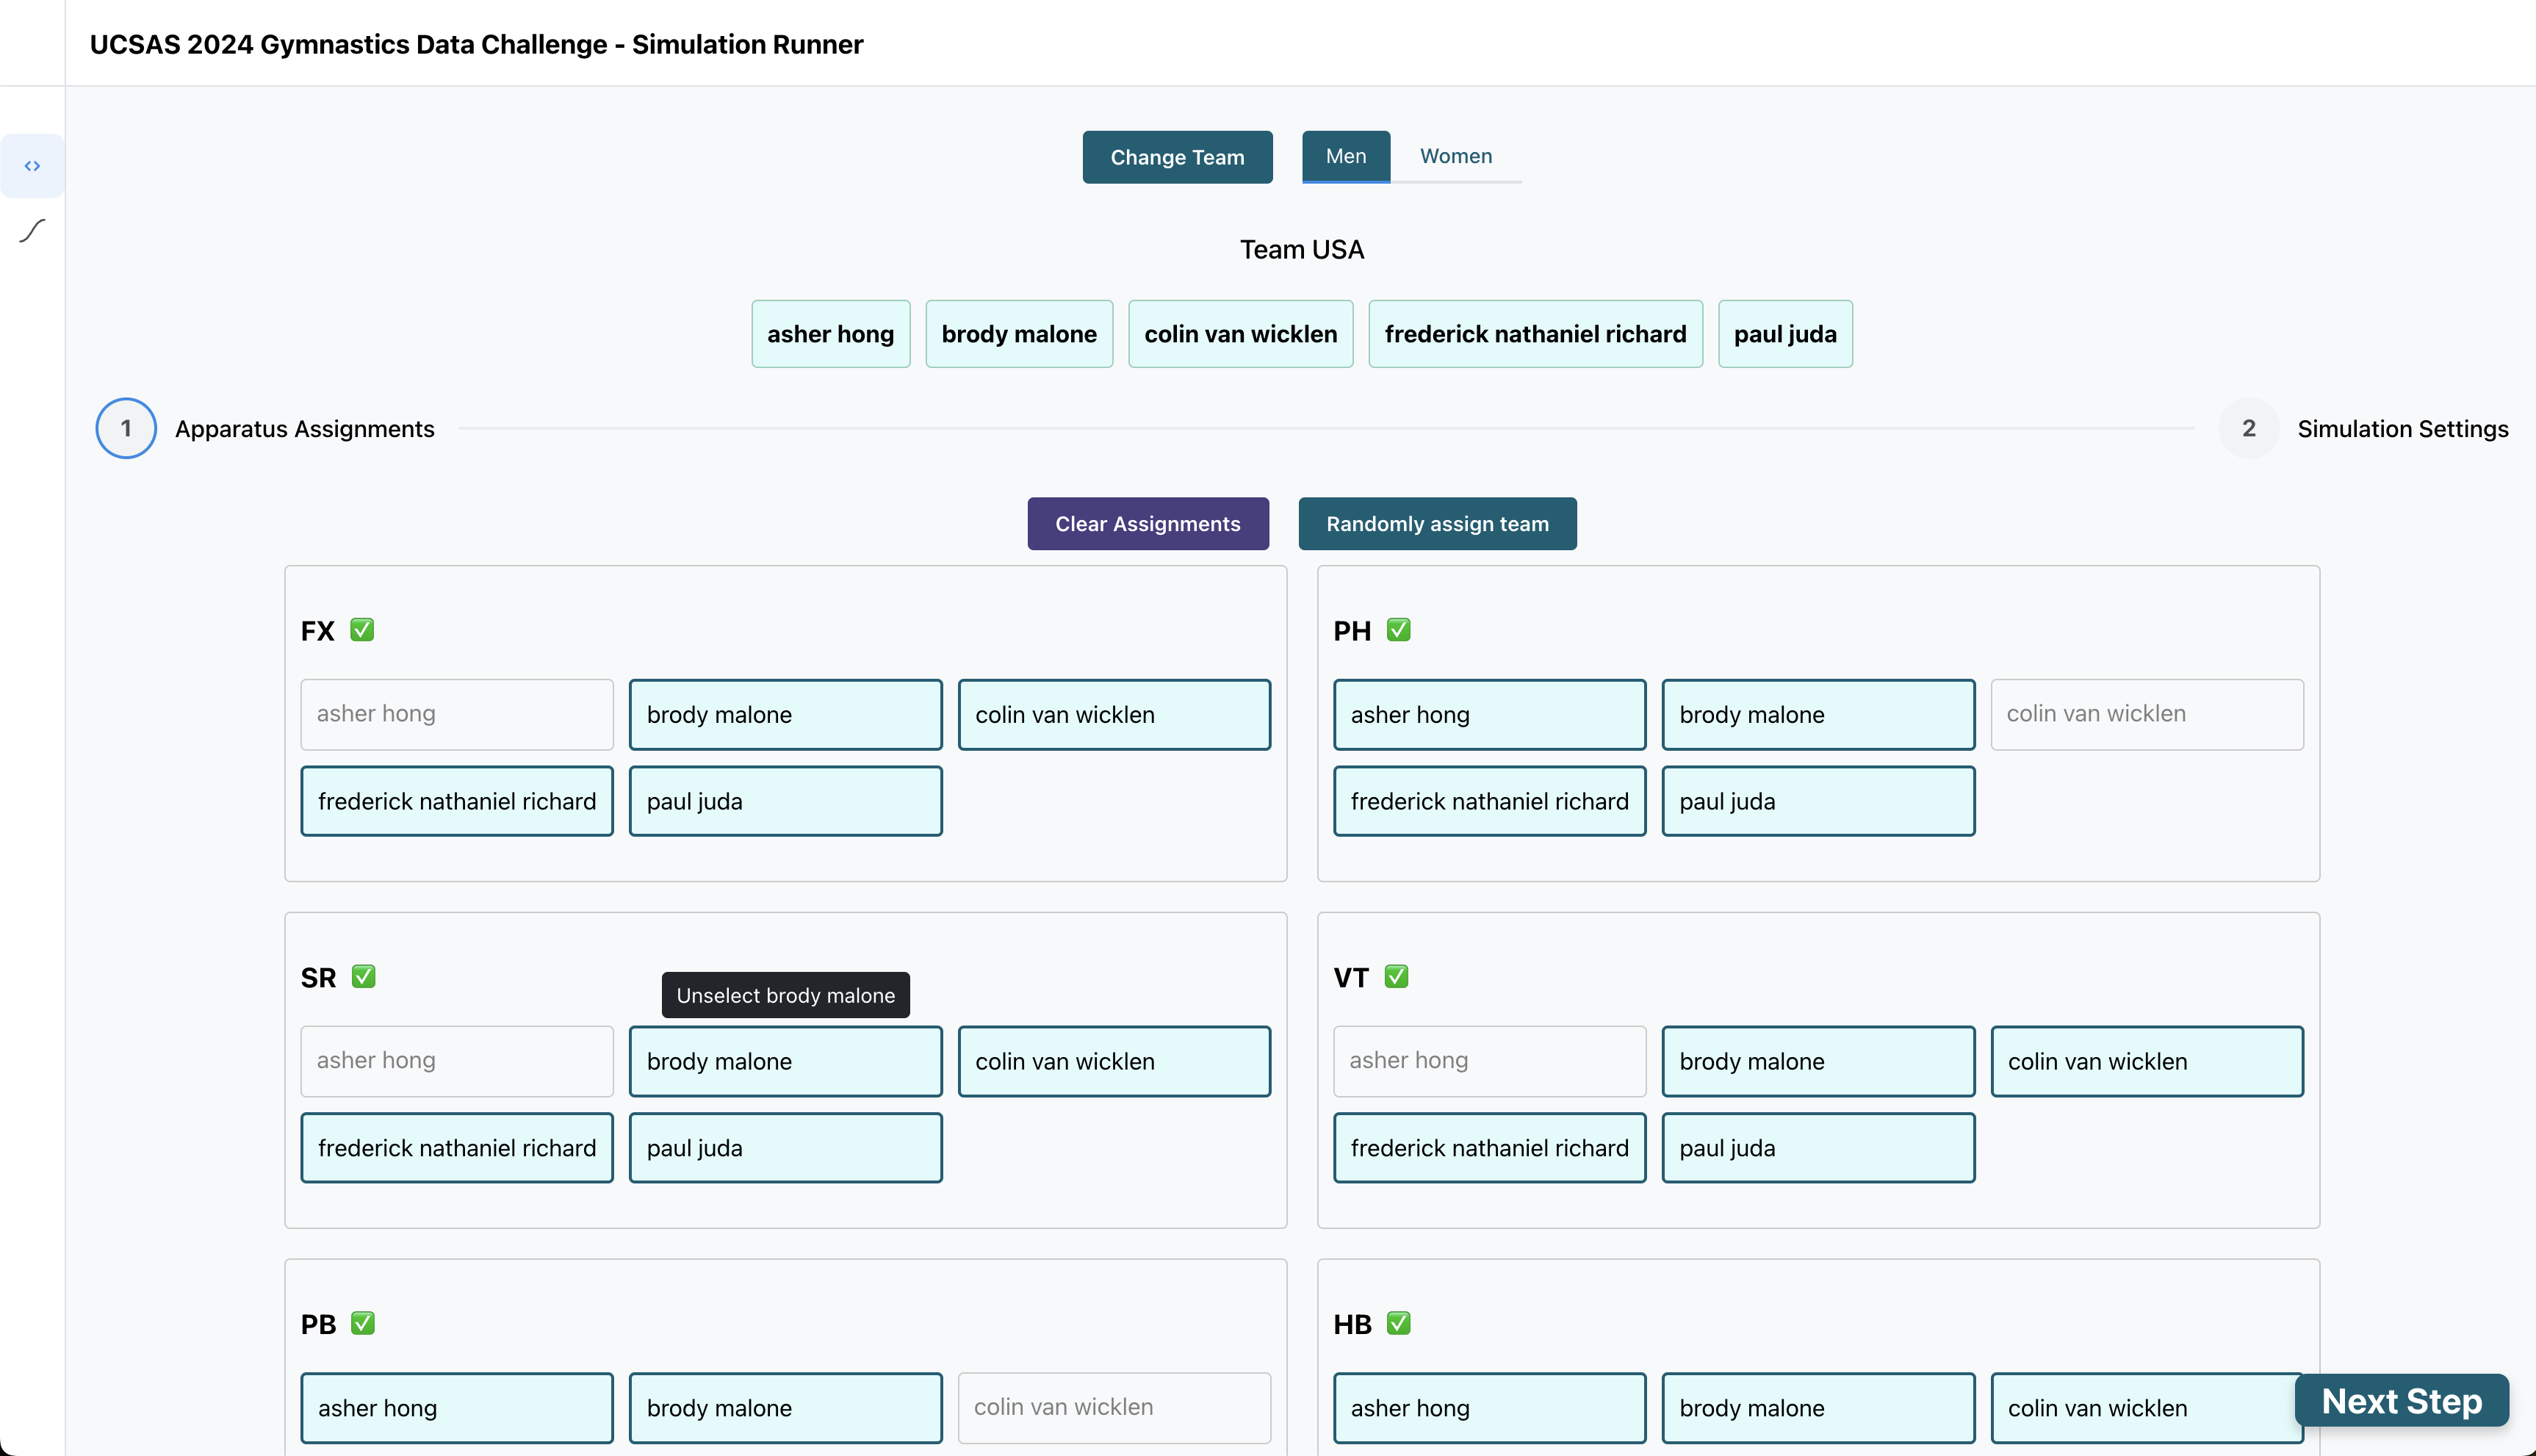
\includegraphics[width=0.8\textwidth]{./simulation_runner.png}
    \caption{Simulation Runner Apparatus Allocations}
    \label{fig:sim_runner}
\end{figure}

\begin{figure}[H]
    \centering
    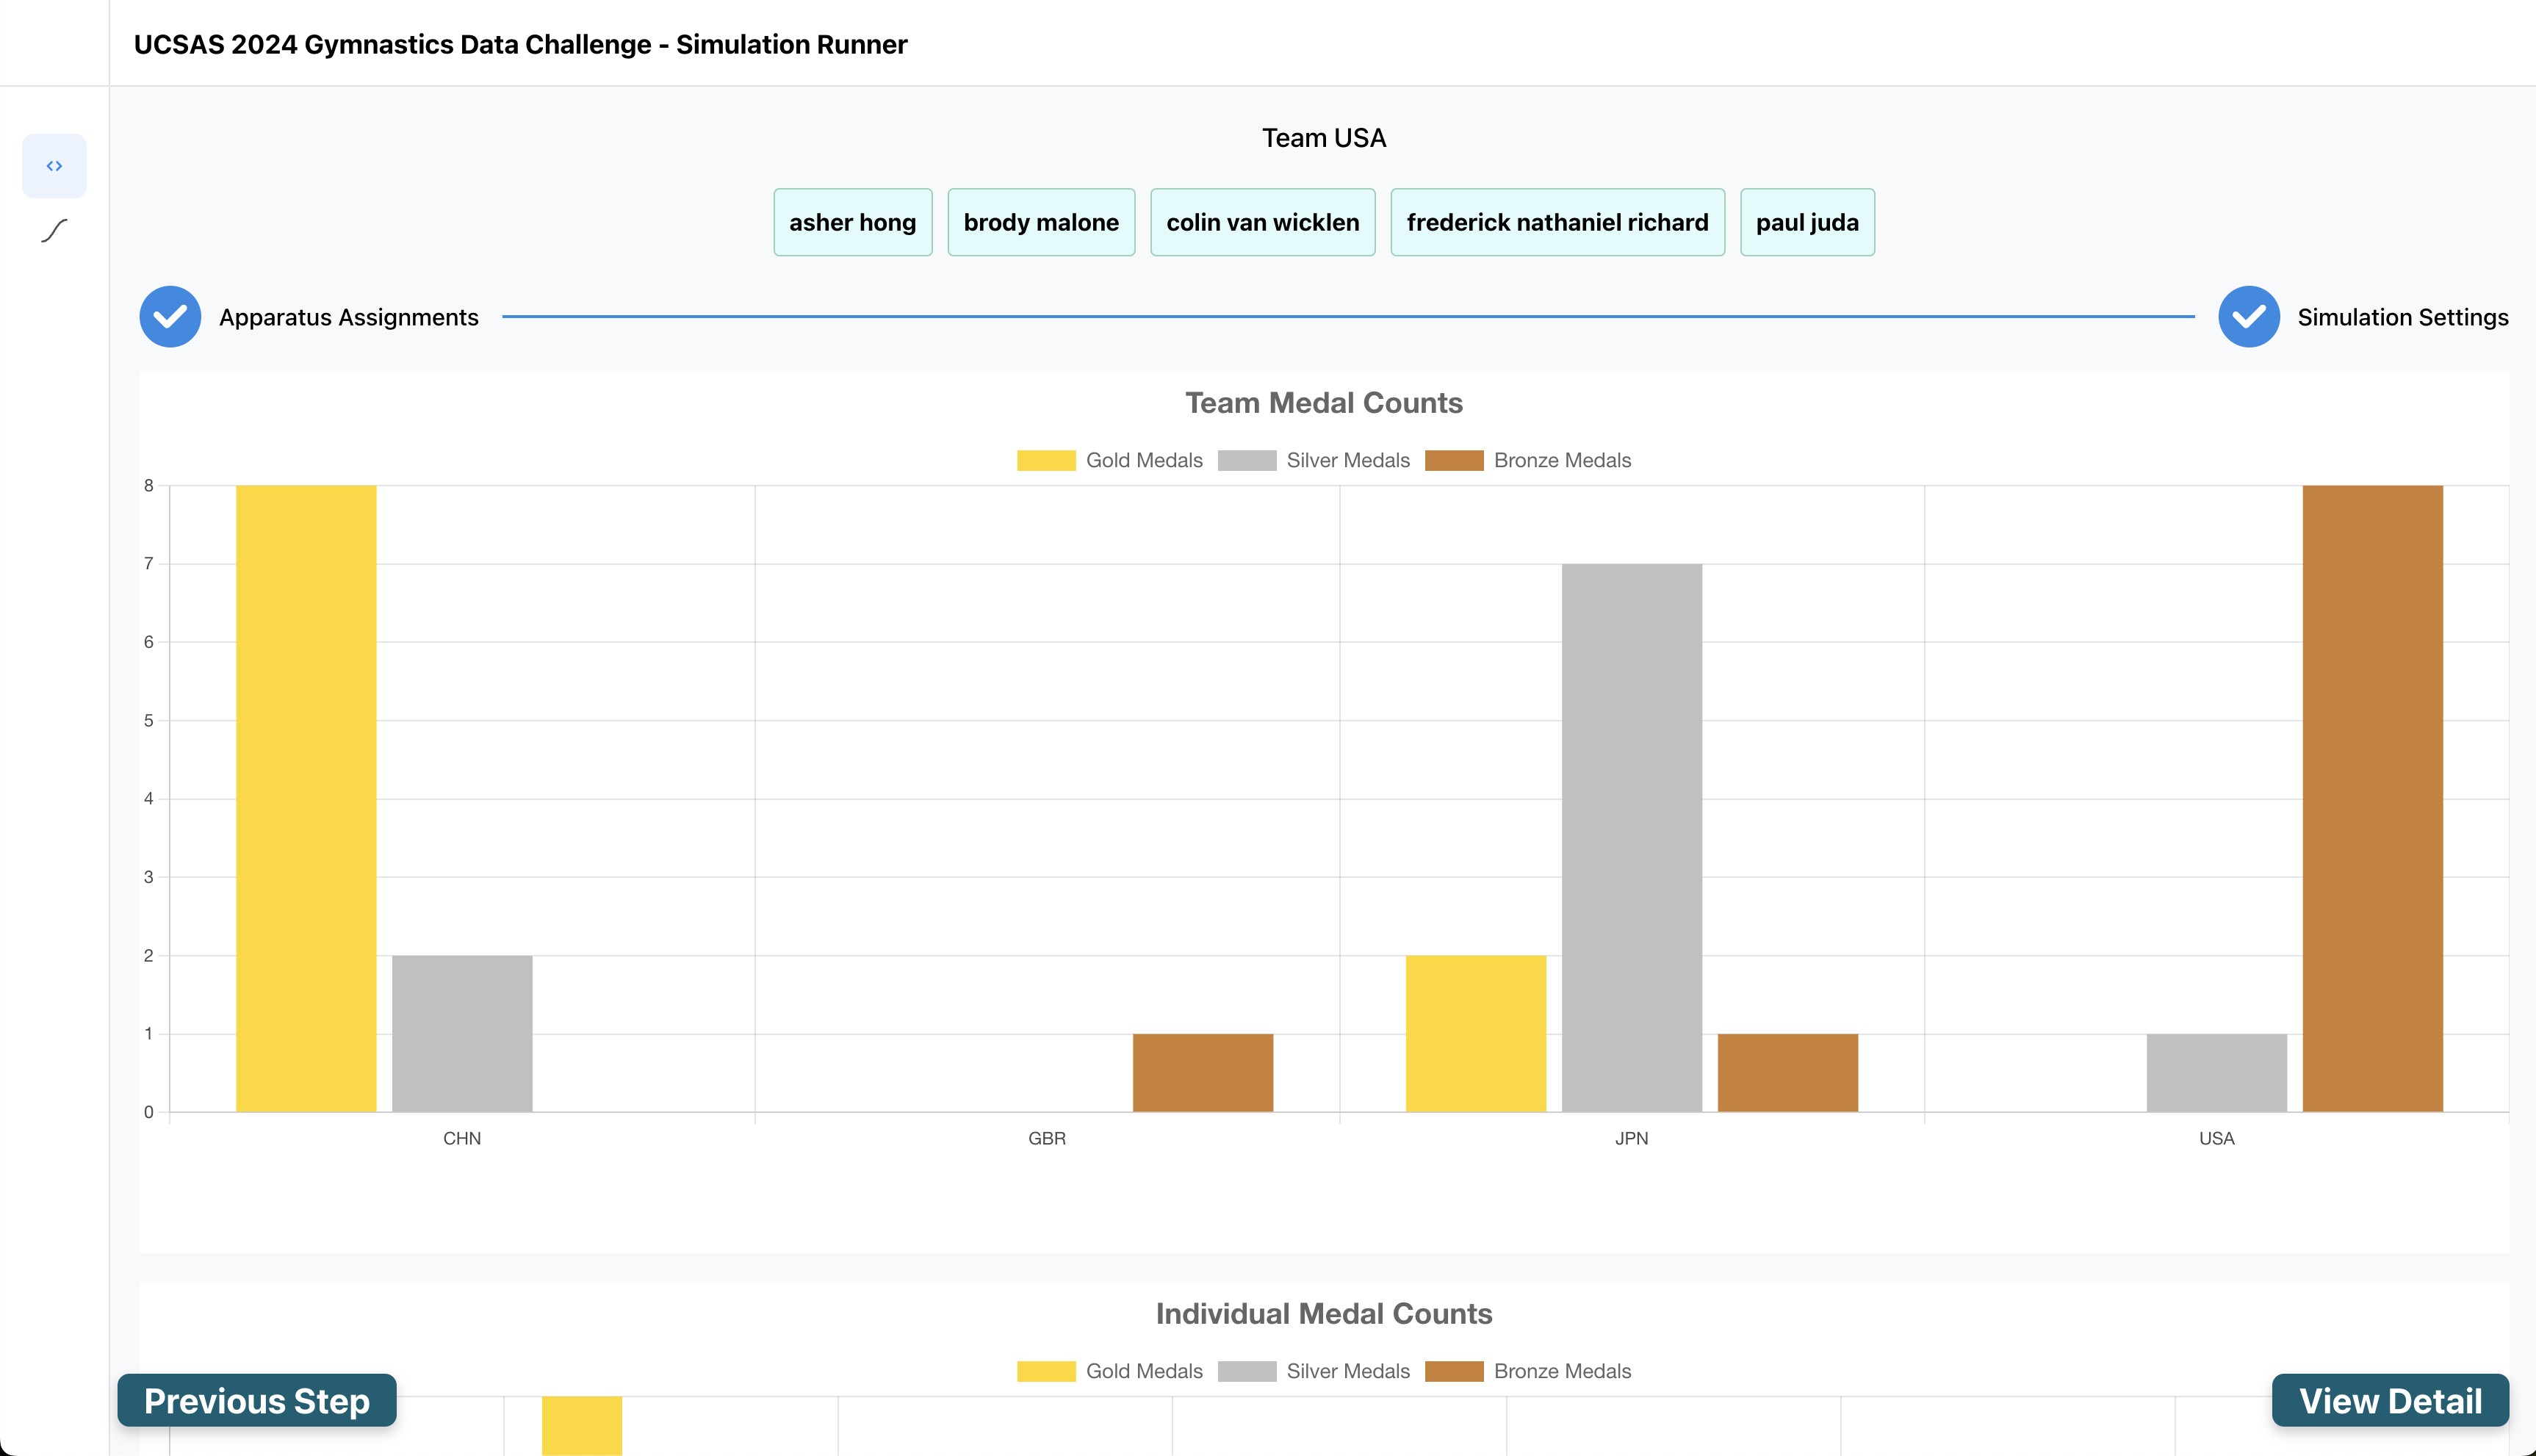
\includegraphics[width=0.8\textwidth]{./results_viewer.png}
    \caption{Simulation Runner Results}
    \label{fig:sim_results}
\end{figure}
\end{document}
